\documentclass{article}%
\usepackage[T1]{fontenc}%
\usepackage[utf8]{inputenc}%
\usepackage{lmodern}%
\usepackage{textcomp}%
\usepackage{lastpage}%
\usepackage[head=40pt,margin=0.5in,bottom=0.6in]{geometry}%
\usepackage{graphicx}%
%
\title{\textbf{Nueva plataforma plantea "proteger la Constitución"}}%
\author{Diario El Universal}%
\date{17/10/2018}%
%
\begin{document}%
\normalsize%
\maketitle%
\textbf{URL: }%
http://www.eluniversal.com/politica/23393/nueva{-}plataforma{-}plantea{-}proteger{-}la{-}constitucion\newline%
%
\textbf{Periodico: }%
EU, %
ID: %
23393, %
Seccion: %
politica\newline%
%
\textbf{Palabras Claves: }%
NO\_TIENE\newline%
%
\textbf{Derecho: }%
CONTEXTO%
, Otros Derechos: %
NO\_TIENE%
, Sub Derechos: %
NO\_TIENE%
\newline%
%
\textbf{EP: }%
NO\newline%
\newline%
%
\textbf{\textit{"Es un gobierno de derecha, neoliberal con características fascistas"}}%
\newline%
\newline%
%
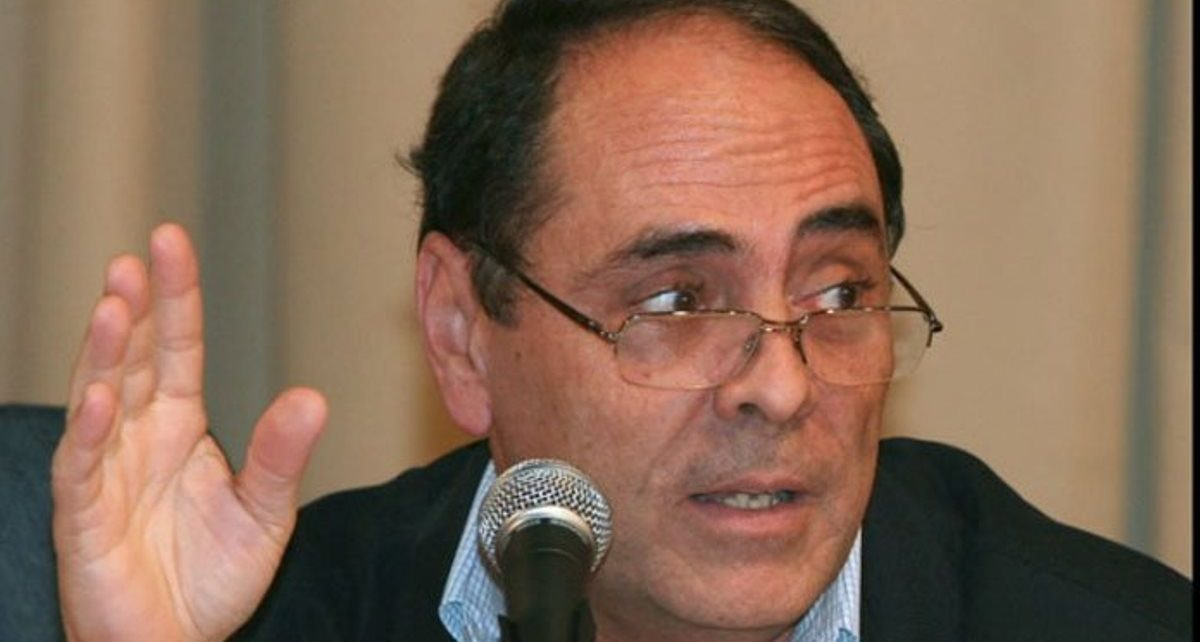
\includegraphics[width=300px]{31.jpg}%
\newline%
%
Los exministros del gobierno del fallecido presidente Hugo Chávez, Héctor Navarro, Ana Elisa Osorio y Oly Millán, conformaron una nueva plataforma política "con el fin de unir fuerzas y defender la Constitución de 1999".%
\newline%
%
Para ello, según apuntaron, prevén llamar a trabajadores y sectores políticos que "no respalden una intervención militar".\newline%
Advierten que se requiere "canalizar el 80\% de rechazo" que, según indican, tiene el Gobierno y evitar que "el Partido Socialista Unido de Venezuela (PSUV) se legitime en el poder para establecer un régimen autoritario".%
\newline%
%
Los exfuncionarios resaltaron que "la abstención no es una opción", ya que abrió las puertas para que "el Gobierno concretara la instalación de una ilegítima Asamblea Nacional Constituyente (ANC)" desde el año pasado.%
\newline%
%
Coincidieron en señalar que "el Gobierno intenta legalizar lo que en la práctica vienen ejecutando, por ello, llaman al país a movilizarse" y a buscar salidas políticas adecuadas.%
\newline%
%
El exministro Héctor Navarro consideró que por sus actuaciones el Gobierno luce inclinado a la "derecha, neoliberal"\newline%
Criticó los recientes casos que a su juicio comprometen los derechos políticos de dirigentes y voces que discrepan con la forma de Gobernar que ejecuta el presidente de la República, Nicolás Maduro.%
\newline%
%
\end{document}